% !TEX root= ../main.tex
\section{Proving inconsistency in graph theories}
\label{sec:Proving inconsistency in graph theories}
We have just shown that in the case of unrestricted theories, we have no guarantee that an inconsistency proof can be constructed using unary and binary NAND-clauses only, so what about graph theories?
After all, it is these theories that motivated the search for this property in the first place.
Unfortunately, it turns out that even for these kinds of theories, there are inconsistency proofs that requires some non-binary NAND-clauses.

We will show this fact by presenting a graph containing a provable binary NAND-clause, an show that the only way to prove it is through using non-binary NAND-clauses.
We will later extend the graph so that it becomes inconsistent, and show that the only way to show this inconsistency is by using the mentioned binary NAND, thus showing that the inconsistency proof must contain a non-binary NAND-clause.

The graph is question is the following:
\[
  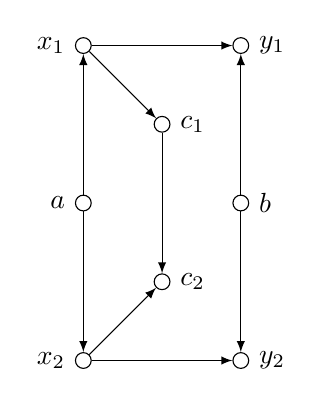
\begin{tikzpicture}
    [
    point/.style={circle,draw,inner sep=0pt,minimum size=2mm},
    collection/.style={thick,rectangle,draw,inner sep=0pt,minimum height=14mm, minimum width= 9mm}
    ]
    \node (a) at (0,2) [point,label=left:$a$] {};
    \node (x1) at (0,4) [point,label=left:$x_1$] {};
    \node (x2) at (0,0) [point,label=left:$x_2$] {};
    \node (b) at (2,2) [point,label=right:$b$] {};
    \node (y1) at (2,4) [point,label=right:$y_1$] {};
    \node (y2) at (2,0) [point,label=right:$y_2$] {};
    \node (c1) at (1,3) [point,label=right:$c_1$] {};
    \node (c2) at (1,1) [point,label=right:$c_2$] {};
    \draw [-latex] (a) to (x1);
    \draw [-latex] (a) to (x2);
    \draw [-latex] (b) to (y1);
    \draw [-latex] (b) to (y2);
    \draw [-latex] (x1) to (y1);
    \draw [-latex] (x1) to (c1);
    \draw [-latex] (x2) to (y2);
    \draw [-latex] (x2) to (c2);
    \draw [-latex] (c1) to (c2);
  \end{tikzpicture}
\]
We will be treating the vertices $y_1$, $y_2$ and $c_2$ in the above graph as if each of them are initial vertices of (non-depicted) disjoint rays, and not sinks, as the figure suggests.
This gives the following axiom set:
\begin{align}
  \text{OR} &= \{ ax_1x_2,\; x_1y_1c_1,\; x_2y_2c_2,\; by_1y_2,\; c_1c_2 \}\\
  \text{NAND} &= \{ \ol{ax_1},\; \ol{ax_2},\; \ol{x_1y_1},\; \ol{x_1c_1},\; \ol{x_2y_2},\; \ol{x_2c_2},\; \ol{by_1},\; \ol{by_2},\; \ol{c_1c_2} \}
\end{align}
Note that we do not include the clauses corresponding to the elements of the above-mentioned rays, since these will not contribute to any useful results\todo{This needs an explanation}.

The NAND-clause that we want to prove is $\ol{ab}$, and this is one way to prove it in Neg:
\begin{prooftree*}
  \Hypo{\ol{ax_2}}
  \Hypo{\ol{by_2}}
  \Hypo{\ol{c_1c_2}}
  \Infer[left label = $x_2y_2c_2$]3{\ol{abc_1}}
  \Hypo{\ol{ax_1}}
  \Hypo{\ol{by_1}}
  \Hypo{\ol{c_1c_2}}
  \Infer[right label = $x_1y_1c_1$]3{\ol{abc_2}}
  \Infer[left label = $c_1c_2$]2{\ol{ab}}
\end{prooftree*}
In the premise of the last step in this proof, we have two non-binary NAND-clauses.
How do we know that this cannot be avoided?

By taking a closer look at the graph, we can work out these 6 solutions (black vertices being assigned 1, while white vertices being assigned 0):

\[
  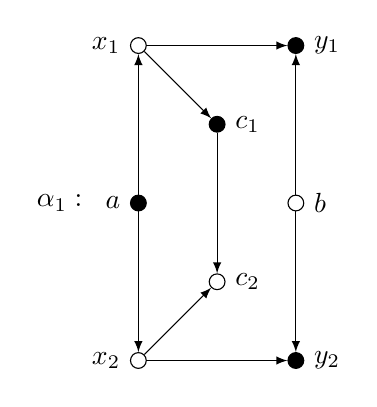
\begin{tikzpicture}
    [
    point/.style={circle,draw,inner sep=0pt,minimum size=2mm},
    one/.style={fill=black},
    collection/.style={thick,rectangle,draw,inner sep=0pt,minimum height=14mm, minimum width= 9mm}
    ]
    \node (label) at (-1,2) {$\alpha_1:$};
    \node (a) at (0,2) [point, one,label=left:$a$] {};
    \node (x1) at (0,4) [point,label=left:$x_1$] {};
    \node (x2) at (0,0) [point,label=left:$x_2$] {};
    \node (b) at (2,2) [point,label=right:$b$] {};
    \node (y1) at (2,4) [point, one,label=right:$y_1$] {};
    \node (y2) at (2,0) [point, one,label=right:$y_2$] {};
    \node (c1) at (1,3) [point, one,label=right:$c_1$] {};
    \node (c2) at (1,1) [point,label=right:$c_2$] {};
    \draw [-latex] (a) to (x1);
    \draw [-latex] (a) to (x2);
    \draw [-latex] (b) to (y1);
    \draw [-latex] (b) to (y2);
    \draw [-latex] (x1) to (y1);
    \draw [-latex] (x1) to (c1);
    \draw [-latex] (x2) to (y2);
    \draw [-latex] (x2) to (c2);
    \draw [-latex] (c1) to (c2);
  \end{tikzpicture}
  \hspace{5mm}
  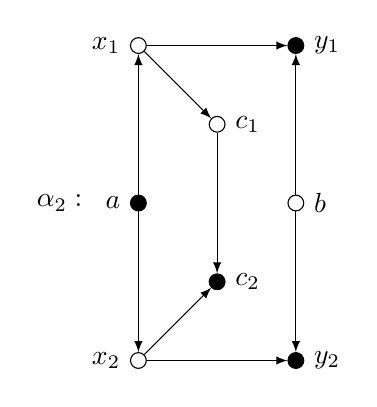
\begin{tikzpicture}
    [
    point/.style={circle,draw,inner sep=0pt,minimum size=2mm},
    one/.style={fill=black},
    collection/.style={thick,rectangle,draw,inner sep=0pt,minimum height=14mm, minimum width= 9mm}
    ]
    \node (label) at (-1,2) {$\alpha_2:$};
    \node (a) at (0,2) [point, one,label=left:$a$] {};
    \node (x1) at (0,4) [point,label=left:$x_1$] {};
    \node (x2) at (0,0) [point,label=left:$x_2$] {};
    \node (b) at (2,2) [point,label=right:$b$] {};
    \node (y1) at (2,4) [point, one,label=right:$y_1$] {};
    \node (y2) at (2,0) [point, one, label=right:$y_2$] {};
    \node (c1) at (1,3) [point,label=right:$c_1$] {};
    \node (c2) at (1,1) [point, one, label=right:$c_2$] {};
    \draw [-latex] (a) to (x1);
    \draw [-latex] (a) to (x2);
    \draw [-latex] (b) to (y1);
    \draw [-latex] (b) to (y2);
    \draw [-latex] (x1) to (y1);
    \draw [-latex] (x1) to (c1);
    \draw [-latex] (x2) to (y2);
    \draw [-latex] (x2) to (c2);
    \draw [-latex] (c1) to (c2);
  \end{tikzpicture}
  \hspace{5mm}
  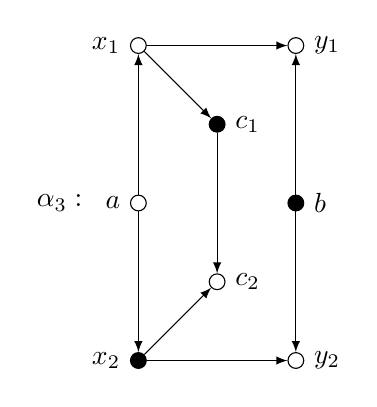
\begin{tikzpicture}
    [
    point/.style={circle,draw,inner sep=0pt,minimum size=2mm},
    one/.style={fill=black},
    collection/.style={thick,rectangle,draw,inner sep=0pt,minimum height=14mm, minimum width= 9mm}
    ]
    \node (label) at (-1,2) {$\alpha_3:$};
    \node (a) at (0,2) [point,label=left:$a$] {};
    \node (x1) at (0,4) [point,label=left:$x_1$] {};
    \node (x2) at (0,0) [point, one,label=left:$x_2$] {};
    \node (b) at (2,2) [point, one,label=right:$b$] {};
    \node (y1) at (2,4) [point,label=right:$y_1$] {};
    \node (y2) at (2,0) [point,label=right:$y_2$] {};
    \node (c1) at (1,3) [point, one,label=right:$c_1$] {};
    \node (c2) at (1,1) [point,label=right:$c_2$] {};
    \draw [-latex] (a) to (x1);
    \draw [-latex] (a) to (x2);
    \draw [-latex] (b) to (y1);
    \draw [-latex] (b) to (y2);
    \draw [-latex] (x1) to (y1);
    \draw [-latex] (x1) to (c1);
    \draw [-latex] (x2) to (y2);
    \draw [-latex] (x2) to (c2);
    \draw [-latex] (c1) to (c2);
  \end{tikzpicture}
\]
\[
  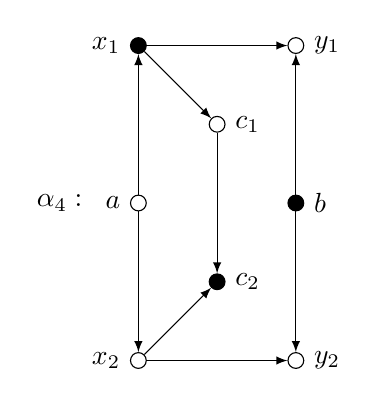
\begin{tikzpicture}
    [
    point/.style={circle,draw,inner sep=0pt,minimum size=2mm},
    one/.style={fill=black},
    collection/.style={thick,rectangle,draw,inner sep=0pt,minimum height=14mm, minimum width= 9mm}
    ]
    \node (label) at (-1,2) {$\alpha_4:$};
    \node (a) at (0,2) [point,label=left:$a$] {};
    \node (x1) at (0,4) [point, one,label=left:$x_1$] {};
    \node (x2) at (0,0) [point,label=left:$x_2$] {};
    \node (b) at (2,2) [point, one,label=right:$b$] {};
    \node (y1) at (2,4) [point,label=right:$y_1$] {};
    \node (y2) at (2,0) [point,label=right:$y_2$] {};
    \node (c1) at (1,3) [point,label=right:$c_1$] {};
    \node (c2) at (1,1) [point, one,label=right:$c_2$] {};
    \draw [-latex] (a) to (x1);
    \draw [-latex] (a) to (x2);
    \draw [-latex] (b) to (y1);
    \draw [-latex] (b) to (y2);
    \draw [-latex] (x1) to (y1);
    \draw [-latex] (x1) to (c1);
    \draw [-latex] (x2) to (y2);
    \draw [-latex] (x2) to (c2);
    \draw [-latex] (c1) to (c2);
  \end{tikzpicture}
  \hspace{5mm}
  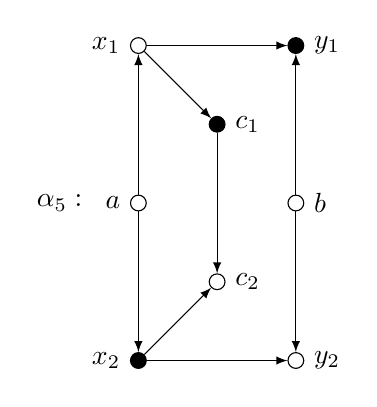
\begin{tikzpicture}
    [
    point/.style={circle,draw,inner sep=0pt,minimum size=2mm},
    one/.style={fill=black},
    collection/.style={thick,rectangle,draw,inner sep=0pt,minimum height=14mm, minimum width= 9mm}
    ]
    \node (label) at (-1,2) {$\alpha_5:$};
    \node (a) at (0,2) [point,label=left:$a$] {};
    \node (x1) at (0,4) [point,label=left:$x_1$] {};
    \node (x2) at (0,0) [point, one,label=left:$x_2$] {};
    \node (b) at (2,2) [point,label=right:$b$] {};
    \node (y1) at (2,4) [point, one, label=right:$y_1$] {};
    \node (y2) at (2,0) [point,label=right:$y_2$] {};
    \node (c1) at (1,3) [point, one,label=right:$c_1$] {};
    \node (c2) at (1,1) [point,label=right:$c_2$] {};
    \draw [-latex] (a) to (x1);
    \draw [-latex] (a) to (x2);
    \draw [-latex] (b) to (y1);
    \draw [-latex] (b) to (y2);
    \draw [-latex] (x1) to (y1);
    \draw [-latex] (x1) to (c1);
    \draw [-latex] (x2) to (y2);
    \draw [-latex] (x2) to (c2);
    \draw [-latex] (c1) to (c2);
  \end{tikzpicture}
  \hspace{5mm}
  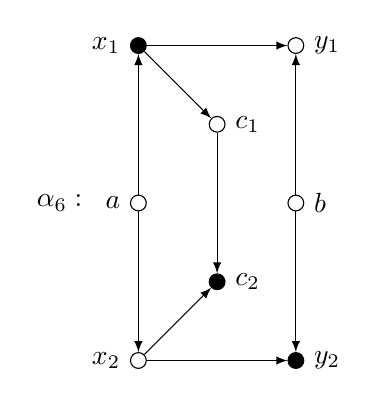
\begin{tikzpicture}
    [
    point/.style={circle,draw,inner sep=0pt,minimum size=2mm},
    one/.style={fill=black},
    collection/.style={thick,rectangle,draw,inner sep=0pt,minimum height=14mm, minimum width= 9mm}
    ]
    \node (label) at (-1,2) {$\alpha_6:$};
    \node (a) at (0,2) [point,label=left:$a$] {};
    \node (x1) at (0,4) [point, one, label=left:$x_1$] {};
    \node (x2) at (0,0) [point,label=left:$x_2$] {};
    \node (b) at (2,2) [point, label=right:$b$] {};
    \node (y1) at (2,4) [point,label=right:$y_1$] {};
    \node (y2) at (2,0) [point, one, label=right:$y_2$] {};
    \node (c1) at (1,3) [point,label=right:$c_1$] {};
    \node (c2) at (1,1) [point, one, label=right:$c_2$] {};
    \draw [-latex] (a) to (x1);
    \draw [-latex] (a) to (x2);
    \draw [-latex] (b) to (y1);
    \draw [-latex] (b) to (y2);
    \draw [-latex] (x1) to (y1);
    \draw [-latex] (x1) to (c1);
    \draw [-latex] (x2) to (y2);
    \draw [-latex] (x2) to (c2);
    \draw [-latex] (c1) to (c2);
  \end{tikzpicture}
\]

Based on these solutions, we can say a lot about the provability of various binary NAND-clauses.
Any pair of vertices from the graph that can be 1 under the same assignment will not be a Neg-provable NAND.
We get this from soundness of Neg, since when two vertices $v$ and $u$ are both 1 under some assignment, we get that $\nvDash \ol{uv}$ and by soundness of Neg that $\nvdash_{Neg} \ol{uv}$.

We can make the following table showing what pairs of vertices can be 1 simultaneously and thus consititute a binary NAND unprovable in Neg.
A cell is filled with a reference to the assignment, if any, examplifying the case.
\[
\begin{array}{|c||c|c|c|c|c|c|c|c|}
  \hline
  & a & b & x_1 & x_2 & y_1 & y_2 & c_1 & c_2 \\ \hline\hline
  a & - & & & & \alpha_1 & \alpha_1 & \alpha_1 & \alpha_2 \\ \hline
  b & & - & \alpha_4 & \alpha_3 & & & \alpha_3 & \alpha_4 \\ \hline
  x_1 & & & - & & & \alpha_6 & & \alpha_6 \\ \hline
  x_2 & & & & - & \alpha_5 & & \alpha_5 & \\ \hline
  y_1 & & & & & - & \alpha_1 & \alpha_1 & \alpha_2 \\ \hline
  y_2 & & & & & & - & \alpha_1 & \alpha_2 \\ \hline
  c_1 & & & & & & & - & \\ \hline
  c_2 & & & & & & & & - \\ \hline
\end{array}
\]

Among the pairs above that are not shown to be unprovable, only two of them are not in the axiom set; $\ol{ab}$ and $\ol{xy}$.
We will use this observation to show that it is impossible to prove $\ol{ab}$ with binary NAND-clauses only.

Let us assume that we have a rule application with all unary or binary NAND-clauses in the premise and with $\ol{ab}$ in the conclusion.
Based on the (Rneg)-rule, we know that the premise must contain at least one binary NAND-clause containg $a$ and at least one containing $b$.
The table above tells us that the only provable binary NAND-clauses that contain $a$ or $b$ are the ones in the axiom set:
$\ol{ax_1}$, $\ol{ax_2}$, $\ol{by_1}$ and $\ol{by_2}$.
Since we don't want any $x_i$ or $y_i$ in the conclusion, these variables has to be removed by the OR-clause.
The OR-clauses $x_1y_1c_1$ and $x_2y_2c_2$ are the only ones that contains both an $x$ and a $y$, making them the only OR-clauses that can potentially conclude with $\ol{ab}$.
This gives us the following information: since both the possible OR-clauses are of length 3, the rule application concluding with $\ol{ab}$ has 3 NAND-clauses in its premise; one containing an $x$, one containing a $y$ and one containing a $c$.
Looking at our table again, we see that the potentially provable NAND-clauses containing a $c$ are again the axioms only.
Since there are no provable NAND-clauses on the form $ac_i$ or $bc_i$, we get that the conclusion of our rule cannot possibly be of length 2, thus contradicting our assumption.
We can therefore conclude that $\ol{ab}$ cannot be proven in Neg using unary and binary NAND-clauses only.

Consider now the following extension of our original graph:

\[
  \begin{tikzpicture}
    [
    point/.style={circle,draw,inner sep=0pt,minimum size=2mm},
    collection/.style={thick,rectangle,draw,inner sep=0pt,minimum height=14mm, minimum width= 9mm}
    ]
    \node (a) at (0,2) [point,label=left:$a$] {};
    \node (x1) at (0,4) [point,label=left:$x_1$] {};
    \node (x2) at (0,0) [point,label=left:$x_2$] {};
    \node (b) at (2,2) [point,label=right:$b$] {};
    \node (y1) at (2,4) [point,label=right:$y_1$] {};
    \node (y2) at (2,0) [point,label=right:$y_2$] {};
    \node (c1) at (1,3) [point,label=right:$c_1$] {};
    \node (c2) at (1,1) [point,label=right:$c_2$] {};
    \node (s) at (1,6) [point,label=left:$s$] {};
    \node (t) at (1,5) [point,label=below:$t$] {};
    \node (u1) at (-2,5) [point,label=left:$u_1$] {};
    \node (u2) at (4,5) [point,label=right:$u_2$] {};
    \draw [-latex] (a) to (x1);
    \draw [-latex] (a) to (x2);
    \draw [-latex] (b) to (y1);
    \draw [-latex] (b) to (y2);
    \draw [-latex] (x1) to (y1);
    \draw [-latex] (x1) to (c1);
    \draw [-latex] (x2) to (y2);
    \draw [-latex] (x2) to (c2);
    \draw [-latex] (c1) to (c2);
    \draw [-latex,loop right] (s) to (s);
    \draw [-latex] (s) to (t);
    \draw [-latex] (t) to (u1);
    \draw [-latex] (t) to (u2);
    \draw [-latex] (u1) to (a);
    \draw [-latex] (u2) to (b);
  \end{tikzpicture}
\]
The extension provides us with 6 new NAND-clauses and 4 new OR-clauses in the axioms set:
\begin{align}
  \text{OR'} &= \text{OR} \cup \{st,\; tu_1u_2,\; u_1a,\; u_2b \}\\
  \text{NAND'} &= \text{NAND} \cup \{\ol{s},\; \ol{st},\; \ol{tu_1},\; \ol{tu_2},\; \ol{u_1a},\; \ol{u_2b} \}
\end{align}

This extended graph can now be proven inconsistent using the newly provided clauses, as shown in the following Neg proof:
\begin{prooftree*}
  \Hypo{\ol{s}}
  \Hypo{\ol{tu_2}}
  \Hypo{\ol{tu_1}}
  \Hypo{\dots}
  \Infer1{\ol{ab}}
  \Infer[right label=$u_1a$]2{\ol{tb}}
  \Infer[right label=$u_2b$]2{\ol{t}}
  \Infer[right label=$st$]2{\varnothing}
\end{prooftree*}

We will now show that this inconsistency proof has to use the $\ol{ab}$ clause.
